\section{Methodology}
\label{sec:methodology}

\subsection{Data Source}

This study utilised the publicly available Emotion Dataset from Kaggle~\citep{emotions_kaggle}, a large-scale collection of Twitter posts annotated into six discrete emotion categories: anger, joy, sadness, fear, surprise, and love. The dataset comprises 416,809 labelled text samples, making it statistically robust for supervised multi-class classification modelling.

The dataset was methodologically justified on three grounds. First, its large sample size enhances statistical reliability and reduces variance in model estimation. Second, it reflects informal, real-world social media language --- including abbreviations, emotive expressions, and conversational tone --- thereby increasing ecological validity. Third, its six-class taxonomy enables fine-grained emotional analysis beyond binary sentiment polarity, directly aligning with the research objective of multi-class emotion prediction.

Each instance consists of a raw textual input (\texttt{text}) and a corresponding encoded emotion label (\texttt{label}). Table~\ref{tab:data_dict} presents the data dictionary.

\begin{table}[!htb]
\centering
\caption{Data dictionary --- Kaggle Emotions Dataset.}
\label{tab:data_dict}
\small
\begin{tabular}{@{}llll@{}}
\toprule
\textbf{Column} & \textbf{dtype} & \textbf{Role} & \textbf{Description} \\
\midrule
\texttt{index} & int & Index & Row identifier \\
\texttt{text} & object & Input & Raw Twitter post text \\
\texttt{label} & int64 & Target & Encoded emotion class \\
\bottomrule
\end{tabular}
\end{table}

The label encoding follows: 0\,=\,Sadness, 1\,=\,Joy, 2\,=\,Love, 3\,=\,Anger, 4\,=\,Fear, 5\,=\,Surprise. Table~\ref{tab:sample_records} presents five representative records drawn from the dataset.

\begin{table}[!htb]
\centering
\caption{Sample records from the Kaggle Emotions Dataset.}
\label{tab:sample_records}
\footnotesize
\setlength{\tabcolsep}{3pt}
\begin{tabular}{@{}clc@{}}
\toprule
\textbf{Idx} & \textbf{Text (sample content)} & \textbf{Label} \\
\midrule
0 & i feel really helpless and heavy hearted & 4 (Fear) \\
1 & ive enjoyed being able to slouch about\ldots & 0 (Sadness) \\
2 & i gave up my internship\ldots feeling lost & 4 (Fear) \\
3 & i dont know i feel so lost & 0 (Sadness) \\
4 & i am a kindergarten teacher\ldots dedicated & 4 (Fear) \\
\bottomrule
\end{tabular}
\end{table}

\subsection{Exploratory Data Analysis}

The objective of EDA was fourfold: (1)~characterise class distribution and quantify imbalance to inform balancing strategies; (2)~examine text length and word count distributions to guide feature engineering and sequence padding decisions; (3)~investigate correlations among numerical features to assess redundancy; and (4)~identify preprocessing requirements arising directly from observed data characteristics.

\subsubsection{Class Distribution Analysis}

Figure~\ref{fig:class_dist} shows the absolute counts per class alongside the proportional breakdown. The distribution revealed a significant imbalance: Joy and Sadness together accounted for nearly 63\% of all samples, while Surprise represented fewer than 4\%. Table~\ref{tab:class_dist} presents the full class distribution with modelling implications.

\begin{figure}[!htb]
\centering
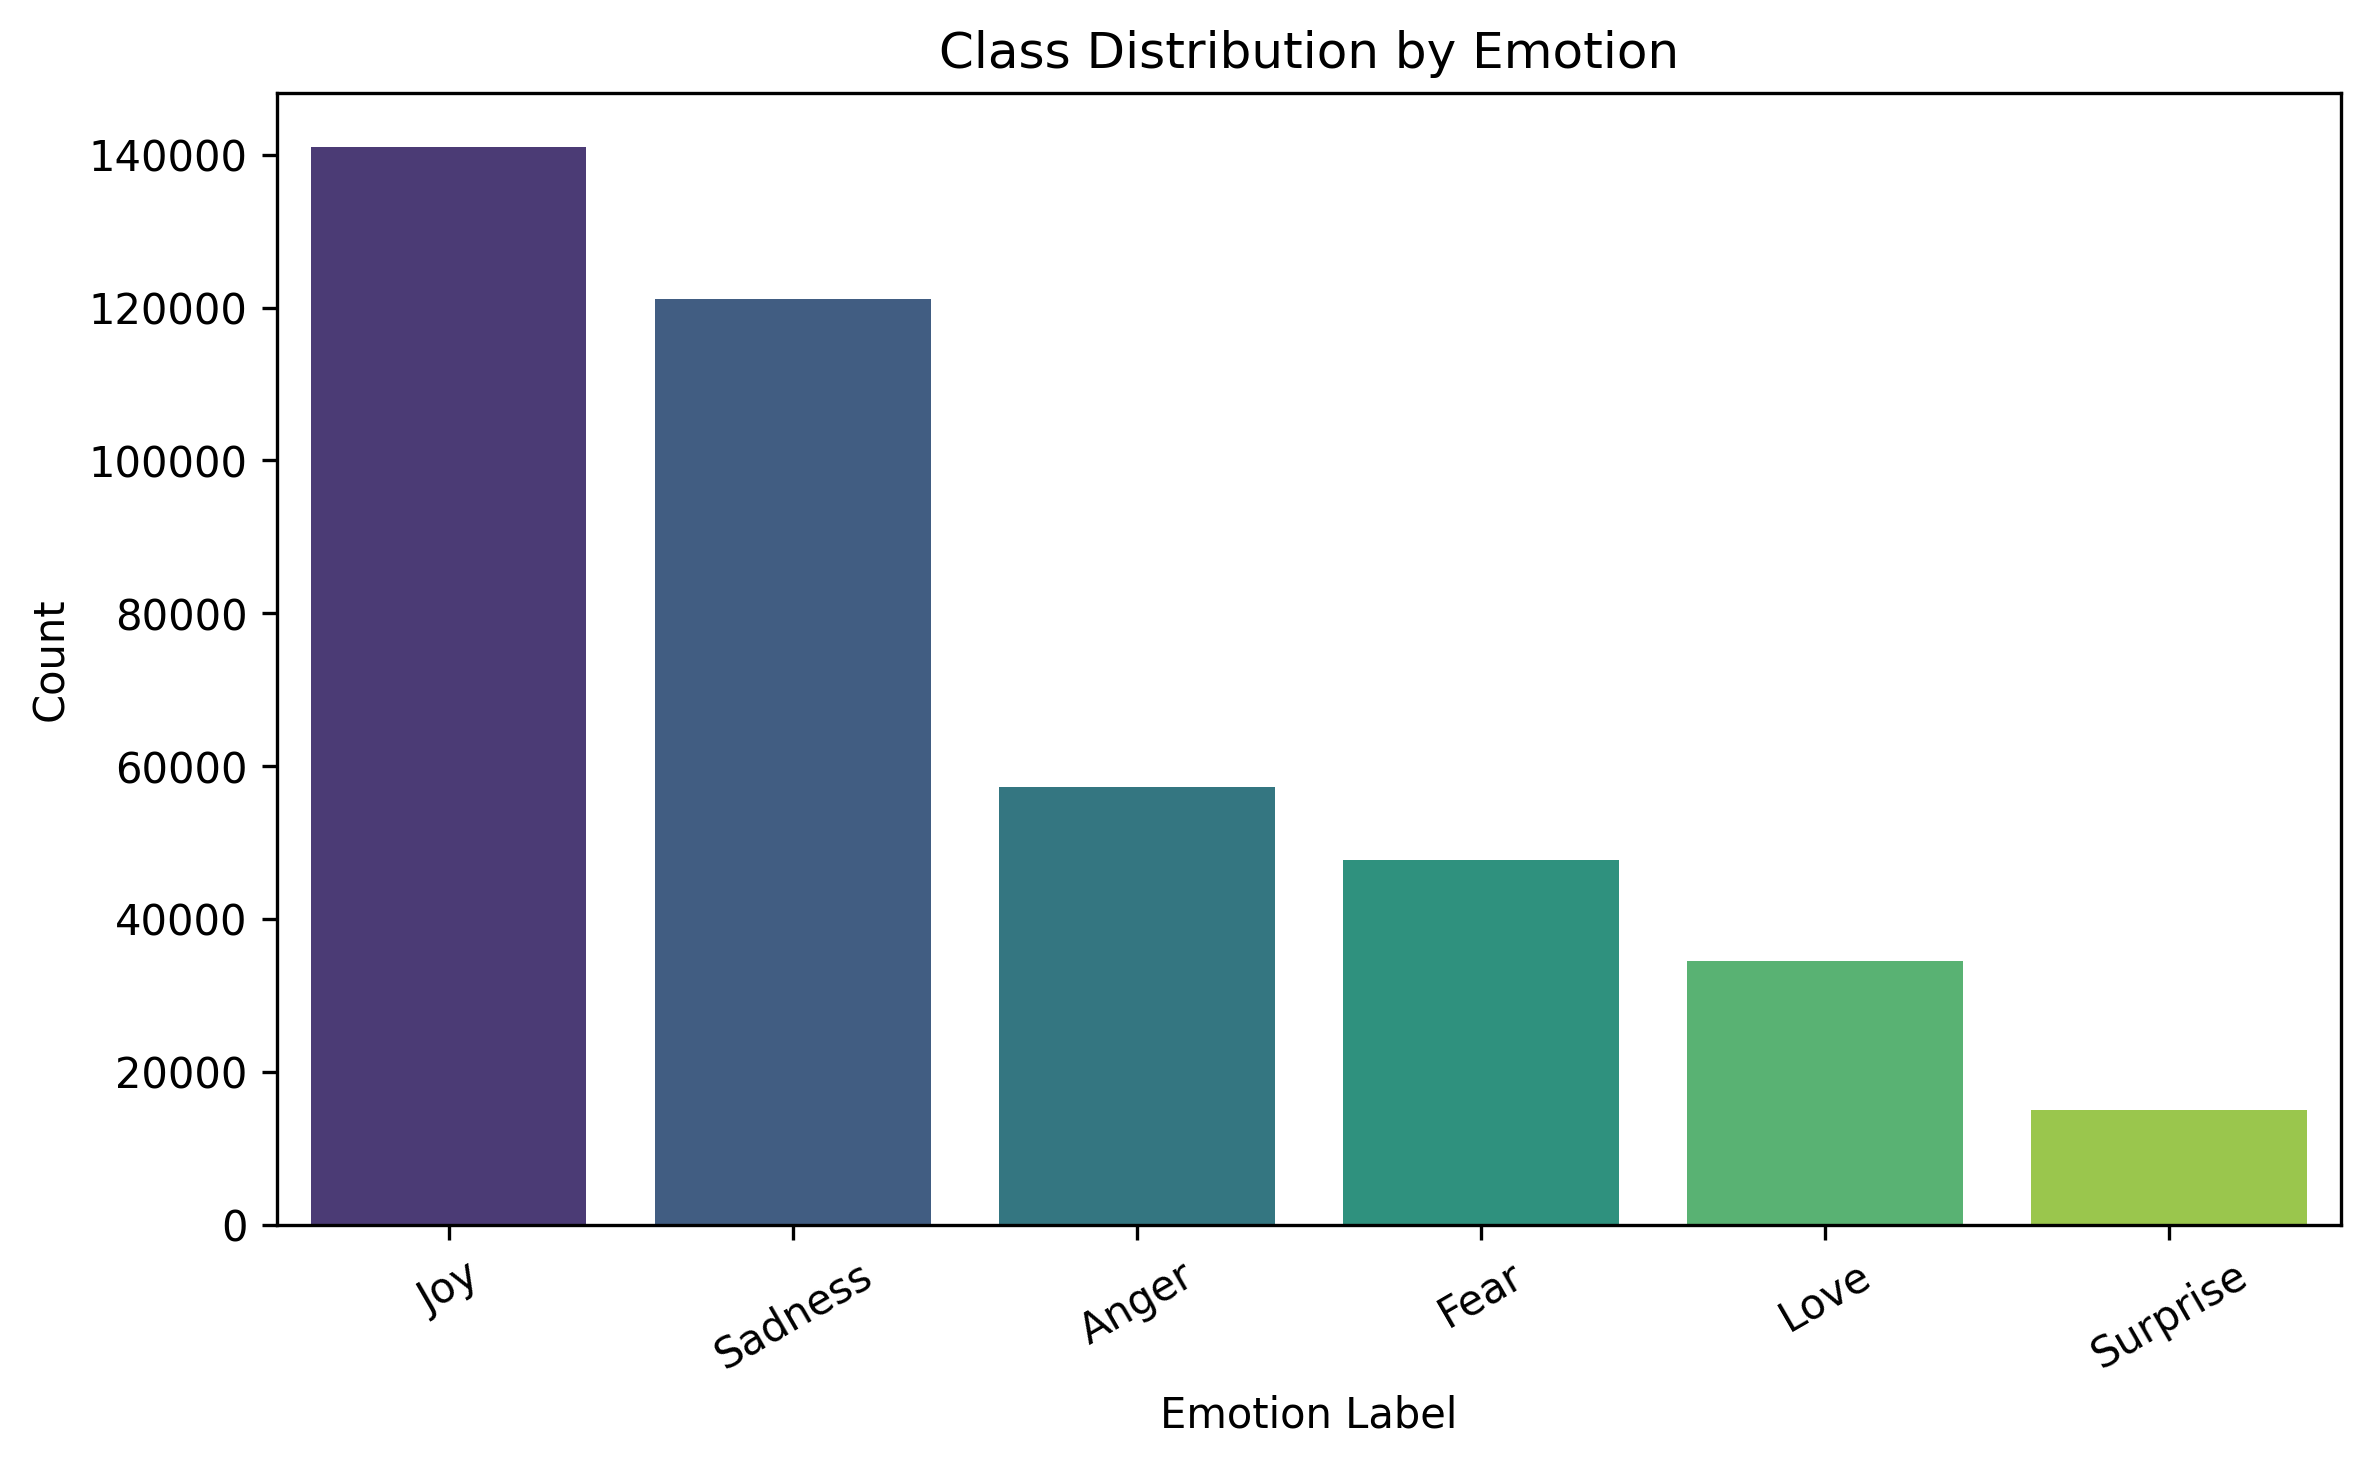
\includegraphics[width=\linewidth]{figures/class_distribution.png}
\caption{Class distribution by emotion label. Joy dominates at 33.8\%, while Surprise is the smallest class at 3.6\%.}
\label{fig:class_dist}
\end{figure}

\begin{table}[!htb]
\centering
\caption{Target variable distribution --- emotion class frequencies and modelling implications.}
\label{tab:class_dist}
\small
\begin{tabular}{@{}clrrl@{}}
\toprule
\textbf{Code} & \textbf{Emotion} & \textbf{Count} & \textbf{\%} & \textbf{Note} \\
\midrule
1 & Joy & 141{,}067 & 33.84 & Largest class \\
0 & Sadness & 121{,}187 & 29.07 & Second largest \\
3 & Anger & 57{,}317 & 13.75 & Mid-tier \\
4 & Fear & 47{,}712 & 11.45 & Overlap w/ Surprise \\
2 & Love & 34{,}554 & 8.29 & Minority class \\
5 & Surprise & 14{,}872 & 3.59 & Highest misclass.\ risk \\
\midrule
  & \textbf{Total} & \textbf{416{,}809} & & IR $\approx$ 9.5\,:\,1 \\
\bottomrule
\end{tabular}
\end{table}

\subsubsection{Text Length and Word Count Distribution}

Figure~\ref{fig:text_length} presents the text length histogram and Figure~\ref{fig:wordcount} shows the word count boxplot by emotion class. The overall median text length was 86 characters (mean 97.0, std 56.2), with Love having the longest posts (median 94 characters) and Anger the shortest (median 84 characters). The histogram confirmed a right-skewed distribution with posts concentrated between 20 and 150 characters. The word count boxplot revealed similar per-class trends, with Love producing the most verbose posts and Anger the most concise. These findings informed the maximum sequence length (512) and padding strategies for neural network architectures.

\begin{figure*}[!htbp]
\centering
\begin{minipage}{0.48\textwidth}
  \centering
  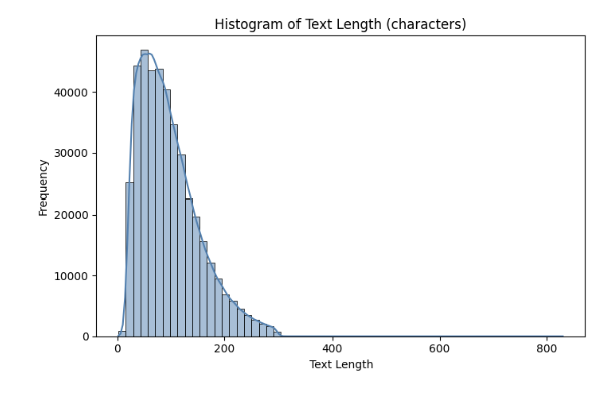
\includegraphics[width=\linewidth]{figures/text_length_wordcount_1.png}
  \captionof{figure}{Histogram of text length distribution.}
  \label{fig:text_length}
\end{minipage}\hfill
\begin{minipage}{0.48\textwidth}
  \centering
  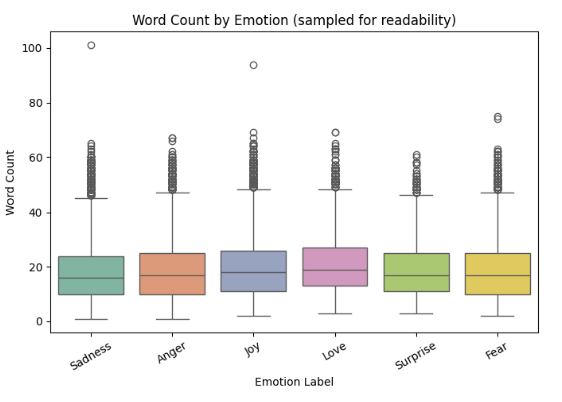
\includegraphics[width=\linewidth]{figures/text_length_wordcount_2.png}
  \captionof{figure}{Word count boxplot by emotion class.}
  \label{fig:wordcount}
\end{minipage}
\end{figure*}

\subsubsection{Correlation Analysis}

A Pearson correlation analysis revealed a strong positive correlation ($r = 0.984$) between \texttt{text\_length} and \texttt{word\_count}, confirming structural redundancy. The correlation between the numeric label encoding and length-based features was near-zero ($r < 0.03$), confirming that emotional classification depends on semantic content rather than message length, reinforcing TF-IDF and embedding-based representations as the essential feature extraction strategy.

\subsection{System Architecture}

The methodology followed a structured NLP workflow: preprocessing $\rightarrow$ feature extraction $\rightarrow$ model development $\rightarrow$ evaluation $\rightarrow$ deployment. The full pipeline is illustrated in Figures~\ref{fig:process_flow} and~\ref{fig:pipeline}.

\textbf{Preprocessing.} An eight-step NLP pipeline normalised raw text: (1)~lowercasing, (2)~whitespace stripping, (3)~URL removal, (4)~emoji removal, (5)~special character removal (retaining only \texttt{[a-z\textbackslash s]}), (6)~chat-word expansion (31 common abbreviations), (7)~stopword removal, and (8)~lemmatisation. Stopword removal used the NLTK English stopword list; however, negation words and intensifiers (\eg, ``not'', ``never'', ``very'', ``extremely'') were retained via a custom exception list, as these tokens carry direct emotional polarity and their removal would cause loss of discriminative signal. Class imbalance was addressed through random downsampling to the minority-class size ($\approx$14,972 per class, 89,832 total).

\textbf{Feature Representation.} For machine learning models, TF-IDF vectorisation (\texttt{max\_features=5000}, \texttt{ngram\_range=(1,2)}) transformed text into numerical feature representations capturing both unigrams and bigrams:
\begin{equation}
\text{TF-IDF}(t, d) = \text{TF}(t, d) \times \log\!\left(\frac{N}{\text{DF}(t)}\right)
\label{eq:tfidf}
\end{equation}
where $\text{TF}(t,d)$ is the term frequency, $\text{DF}(t)$ is the document frequency, and $N$ is the total number of documents. For deep learning models, an embedding layer converted tokens into dense vector representations.

\textbf{Data Splitting.} The dataset was split 80\% training / 20\% testing with a 20\% validation holdout from training data, using stratified sampling to preserve class proportions.

\textbf{Evaluation Metrics.} Model performance was evaluated using precision, recall, per-class F1, macro-averaged F1 ($K=6$ classes), and accuracy:
\begin{align}
\text{Precision} &= \frac{TP}{TP + FP} \label{eq:precision}\\
\text{Recall} &= \frac{TP}{TP + FN} \label{eq:recall}\\
F_1 &= \frac{2 \times \text{Precision} \times \text{Recall}}{\text{Precision} + \text{Recall}} \label{eq:f1}\\
\text{Macro-}F_1 &= \frac{1}{K}\sum_{k=1}^{K} F_{1,k} \label{eq:macro_f1}\\
\text{Accuracy} &= \frac{\text{Number of correct predictions}}{\text{Total predictions}} \label{eq:accuracy}
\end{align}

\begin{figure}[!htb]
\centering
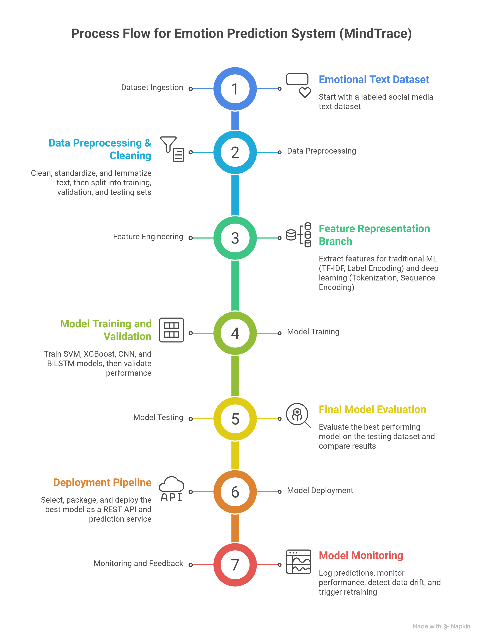
\includegraphics[width=\linewidth]{figures/process_flow.png}
\caption{MindTrace process flow --- from raw dataset through preprocessing, feature extraction, model training, evaluation, and deployment.}
\label{fig:process_flow}
\end{figure}

\begin{figure}[!htb]
\centering
\begin{tikzpicture}[
    node distance=0.4cm and 0.3cm,
    >={Stealth[length=2.5pt]},
    mainbox/.style={rectangle, draw=gray!60, rounded corners=2pt, align=center,
                font=\sffamily\tiny, minimum width=3.4cm,
                minimum height=0.45cm, fill=#1, text width=3.4cm,
                line width=0.4pt},
    mainbox/.default={blue!8},
    featbox/.style={rectangle, draw=gray!60, rounded corners=2pt, align=center,
                font=\sffamily\tiny, minimum width=1.6cm,
                minimum height=0.35cm, fill=#1, text width=1.6cm,
                line width=0.4pt},
    featbox/.default={green!10},
    modelbox/.style={rectangle, draw=gray!60, rounded corners=2pt, align=center,
                font=\sffamily\tiny\bfseries, minimum width=0.9cm,
                minimum height=0.32cm, fill=orange!12, line width=0.4pt},
    arr/.style={->, semithick, color=gray!60},
    plainline/.style={semithick, color=gray!60},
]

% ── Row 1: Dataset ──
\node[mainbox=cyan!10] (data) {
    \textbf{Emotional Text Dataset}\\[-1pt]
    {\tiny 416{,}809 labelled tweets}
};

% ── Row 2: Preprocessing ──
\node[mainbox=blue!8, below=0.4cm of data] (preproc) {
    \textbf{Data Preprocessing}\\[-1pt]
    {\tiny Downsample\,$\cdot$\,Standardise\,$\cdot$\,Lemmatise}
};

% ── Row 3: Feature branches (side by side) ──
\node[featbox=green!10, below left=0.55cm and 0.5cm of preproc] (ml) {
    \textbf{ML Features}\\[-1pt]
    {\tiny TF-IDF Vectoriser}\\[-1pt]
    {\tiny Label Encoder}
};
\node[featbox=violet!10, below right=0.55cm and 0.5cm of preproc] (dl) {
    \textbf{DL Features}\\[-1pt]
    {\tiny Tokenisation}\\[-1pt]
    {\tiny Sequence Padding}
};

% ── Row 4: Data split ──
\node[mainbox=yellow!12, below=1.35cm of preproc] (split) {
    \textbf{Data Splitting}\\[-1pt]
    {\tiny 80\,\% Train (20\,\% Val) \,$\cdot$\, 20\,\% Test}
};

% ── Row 5: Four model boxes ──
\node[modelbox, below=0.55cm of split, xshift=-1.05cm] (svm)    {SVM};
\node[modelbox, right=0.08cm of svm]                    (xgb)    {XGBoost};
\node[modelbox, right=0.08cm of xgb]                    (cnn)    {CNN};
\node[modelbox, right=0.08cm of cnn]                    (bilstm) {BiLSTM};

% ── Row 6: Evaluation ──
\node[mainbox=red!7, below=1.6cm of split] (eval) {
    \textbf{Model Evaluation}\\[-1pt]
    {\tiny Accuracy \,$\cdot$\, F1-Score \,$\cdot$\, Confusion Matrix}
};

% ── Row 7: Deployment ──
\node[mainbox=teal!10, below=0.4cm of eval] (deploy) {
    \textbf{Deployment (SVM)}\\[-1pt]
    {\tiny Flask REST API + Docker + CI/CD}\\[-1pt]
    {\tiny Best accuracy--latency trade-off}
};

% ════════════════ Arrows ════════════════

% Dataset → Preprocessing
\draw[arr] (data.south) -- (preproc.north);

% Preprocessing → branches (T-fork: down, then left/right)
\coordinate (fork) at ($(preproc.south)+(0,-0.18)$);
\draw[plainline] (preproc.south) -- (fork);
\draw[plainline] (fork) -- (fork -| ml.north);
\draw[plainline] (fork) -- (fork -| dl.north);
\draw[arr] (fork -| ml.north) -- (ml.north);
\draw[arr] (fork -| dl.north) -- (dl.north);

% Branches → Split (each goes down then horizontal to split edge)
\coordinate (mlbot) at ($(ml.south)+(0,-0.12)$);
\coordinate (dlbot) at ($(dl.south)+(0,-0.12)$);
\draw[plainline] (ml.south) -- (mlbot);
\draw[arr] (mlbot) -- (mlbot -| split.west) -- (split.west);
\draw[plainline] (dl.south) -- (dlbot);
\draw[arr] (dlbot) -- (dlbot -| split.east) -- (split.east);

% Split → models (T-fork: down, then spread to each model)
\coordinate (mfork) at ($(split.south)+(0,-0.12)$);
\draw[plainline] (split.south) -- (mfork);
\draw[plainline] (mfork -| svm.north) -- (mfork -| bilstm.north);
\draw[arr] (mfork -| svm.north) -- (svm.north);
\draw[arr] (mfork -| xgb.north) -- (xgb.north);
\draw[arr] (mfork -| cnn.north) -- (cnn.north);
\draw[arr] (mfork -| bilstm.north) -- (bilstm.north);

% Models → Evaluation (individual rectangular arrows, funnel inward)
\draw[arr] (svm.south)    -- ++(0,-0.30) -| ($(eval.north)+(-0.6,0)$);
\draw[arr] (xgb.south)    -- ++(0,-0.15) -| ($(eval.north)+(-0.2,0)$);
\draw[arr] (cnn.south)    -- ++(0,-0.15) -| ($(eval.north)+(0.2,0)$);
\draw[arr] (bilstm.south) -- ++(0,-0.30) -| ($(eval.north)+(0.6,0)$);

% Evaluation → Deployment
\draw[arr] (eval.south) -- (deploy.north);

\end{tikzpicture}
\caption{MindTrace end-to-end pipeline architecture.}
\label{fig:pipeline}
\end{figure}
